\chapter{NetShaper: A Differentially-Private Side Channel Mitigation System}
\label{ch:netshaper}

NetShaper \cite{sabzi2024netshaper} is both the name of the framework and the system that implements the framework to mitigate network side-channel attacks in internet applications.
We have provided a brief outline of the framework in \Cref{subsec:netshaper-background-framework}. 
Here, we describe the NetShaper system.

We first outline the requirements that the system should fulfil.
First, in any given window $W$, the system should be able to obtain the size of the payload in the buffering queue, with noise added to it. 
That is, the system should be able to complete the execution of $f_{DP}(S, t_{start}, t_{start} + W)$.
In the same window, the system should also be able to send out the payload, with padding, if necessary, such that the total data sent out, $b_{out}$, is equal to the noised size. 
However, it is sufficient to be able to queue $b_{out}$ bytes to be sent out, even if the actual transmission goes beyond the window $W$, as long as any delays were not caused by the payload coming in or already present in the buffering queue. 
The reason for this is the post-processing property of DP that we outlined in \Cref{subsubsec:netshaper-background-framework-dp}.

Second, the payload and the padding should be indistinguishable to any observer observing the outbound packet stream.
Hence, the payload and padding should both be subject to the same congestion control, re-transmission, loss recovery, and other network behaviour.
In addition, the outbound transmission should provide the same or a higher level of reliability than the applications using this system expect.

Finally, the system should be modular so that modifications to any one sub-component do not require changes in the other components.
The system should also be portable and easily deployable, requiring none to minimal changes on the end hosts where the applications are running.
These goals ascertain that the system is easy to adopt and deploy and can easily be modified per the deployer's requirements.


% 1. Complete DP measurement within the window W
% 2. Data and Dummy should be indistinguishable
% 3. Should provide the same level of reliability the application expects
% 4. Should be modular for easy modification to sub-components
% 5. Should be portable and easily deployable, with minimal modifications of the end-hosts.

% \section{Introduction}
% \label{sec:netshaper-intro}

Encryption, which has become the de-facto mechanism for protecting communication over the internet, does not conceal the shape of the traffic.
Prior work has demonstrated that in many applications, this traffic shape has a strong correlation with the data being transmitted.
For example, webpages on the internet access different resources like CSS, javascript and images in a unique pattern which can be fingerprinted \cite{gong2010fingerprinting, bhat2019varcnn, wang2014supersequence}.
Most videos that are streamed on the internet rely on the DASH standard \cite{dash2013}.
As such, the videos are split into five-second segments, which are compressed individually and transmitted in a burst of traffic every five seconds, which can also be uniquely fingerprinted \cite{schuster2017beautyburst}.
Attacks that exploit this correlation to reveal some information about the traffic being transmitted are known as network side-channel attacks.


In order to mitigate network side-channel attacks, prior work has proposed various methods to modify the shape of the traffic to hide the correlation between the content of the traffic and the packet sizes and timing \cite{hou2020wf, nasr2021blind, rahman2020mockingbird, shan2021dolos, wang2017walkie, wright2009traffic, mehta2022pacer, zhang2019statistical, cai2014csbuflo}.
However, prior work has focused less on the ease of adoption of these solutions. 
Some solutions only rely on simulations and do not provide a functional and deployable system at all \cite{wang2014supersequence, nithyanand2014glove, cai2014tamaraw}. 
Others require non-trivial modifications to the end host and either do no support or do not scale well with multiple users \cite{cai2014csbuflo, mehta2022pacer}.
In addition, None of these systems have a modular design that can be easily extended to support more types of traffic and protocols.

This chapter presents the NetShaper system, a modular, portable, scalable network side-channel mitigation system.
NetShaper is a modular transport layer (L4) proxy tunnel that can be integrated with any network stack and within any node.
Our system only requires the end-host to change their operating systems or browser's proxy configuration.
NetShaper's modular architecture allows easy modification of any system sub-component to support additional protocols or alternative implementations.
In order to support and scale with multiple clients, NetShaper relies on the QUIC protocol and assigns a QUIC stream to every client-server pair.

The rest of the chapter is organised as follows:
In \Cref{sec:netshaper-background}, we first provide a background on network side-channel attacks, how differential privacy can be used to mitigate such attacks, and how the QUIC protocol, which is fundamental to the scalability of NetShaper, works.
In \Cref{sec:netshaper-threat-model}, we outline the Threat Model with which NetShaper works.
We then present the design of NetShaper's QUIC-based traffic shaping tunnel in \Cref{sec:netshaper-designing-traffic-shaping-tunnel}.
\Cref{sec:netshaper-middlebox-implementation} outlines the system implementation of NetShaper.
We evaluate the performance of NetShaper and provide the results in \Cref{sec:netshaper-evaluation}.
We then discuss the limitations of NetShaper in \Cref{sec:netshaper-limitations}.
Finally, we conclude the chapter by providing a comprehensive view of the related work and how NetShaper fares against them in \Cref{sec:netshaper-related-work}.

\endinput

Encryption has become the de-facto mechanism for protecting any communication over the internet. 
While encryption conceals the data being transmitted, it does not conceal the metadata associated with the transmission itself, such as the packet sizes and timing (i.e. the traffic shape).
As such, while encryption can prevent the leakage of data by direct observation of the communication, it does not prevent leaks caused by the observation of the metadata.
\section{Background}
\label{sec:netshaper-background}

\subsection{Network Side Channels}
\label{subsec:netshaper-background-network-side-channels}

Today, people rely on the internet for everyday tasks such as sending a message or calling friends, watching a video or movie, sharing files, accessing their bank accounts, or looking up their medical condition.
As people using the internet may be transmitting or receiving sensitive information, it becomes necessary to protect these transmissions.

While encryption can protect against eavesdroppers interested in obtaining sensitive information, encryption alone is insufficient.
Encryption does not conceal the packet sizes and timing, which can be correlated with the sensitive information of the user. 
An attacker can leverage this correlation to infer the sensitive information solely by observing the network link and obtaining the packet sizes and timing.
Such attacks are called network side-channel attacks.

With a network side-channel attack, an attacker wants to determine the contents of the web traffic being transmitted or received by the victim.
More often than not, an attacker is interested in knowing if the victim accessed any content from a small subset and, if so, which content they accessed.
To do this, the attacker follows these steps: 
1) Collect network traces
2) Build a classifier trained on the collected network traces
3) Gain access to the network shared with the victim
4) Profile the victim's network traffic
5) Determine whether the victim accessed any content of interest to the attacker

First, the attacker builds a collection of the content (e.g. webpages and video streams) that they are interested in. 
They collect network traces for this content under various network conditions to account for variability caused by the network itself. 
Then, the attacker trains a classifier on this collected network trace.
The classifier can use multiple features like packer sizes, inter-packer timing, total bytes transferred in a burst of packets, the duration of the burst and the interval between bursts, and the direction of the bursts \cite{schuster2017beautyburst}.

Now, to carry out the attack, the attacker gains access to some network path shared with the victim.
The attacker could own a router or switch on the network path of the victim, or another machine that shares the same router or switch that the victim is connected to.
If they own an element in the network path, they can directly observe all the features necessary to carry out the attack. 
Otherwise, they create congestion in the shared network path such that the victim's network traffic would contend with the attacker's traffic.
In this case, the attacker's traffic would be delayed, and the delay would be proportional to the victim's traffic, thus revealing some features of the victim's traffic.
The attacker could also have infiltrated the victim's machine, and maybe running a malicious application on that machine.
The malicious application could be a javascript-based advertisement on the page the victim is visiting or another process on the victim's machine, thus gaining the ability to create contention on the network card in the victim's machine. 


Once the attacker has access to the shared network path with the victim, they collect the network traces of their own traffic. and, based on that, extract the features of the victim's traffic flow.
These extracted features are then run through the pre-trained classifier, which helps the attacker determine which content the victim accessed. 
\citet{schuster2017beautyburst} demonstrated that one could train a Convolution Neural Network (CNN)-based classifier to determine which video the victim is streaming.
Similarly, prior work has demonstrated that such a network side-channel attack can also be used to determine which webpage the victim is visiting \cite{hayes2016kfp, panchenko2016website, gong2010fingerprinting}

% \section{Threat Model}\label{sec:nsc-threat-model}

\subsection{Mitigating Network Side Channels using Differential Privacy}
\label{subsec:netshaper-background-framework}

There are many different ways to add noise to network traffic to remove the correlation between the content of the traffic and the shape of the traffic.
However, most approaches either have a high overhead or high latency \cite{cai2014csbuflo, mehta2022pacer} or do not provide any meaningful privacy guarantees \cite{hou2020wf, nasr2021blind, rahman2020mockingbird, shan2021dolos, wang2017walkie, wright2009traffic}.
Here, we briefly describe the NetShaper framework that addresses all of these concerns.
NetShaper's framework relies on Differential Privacy (DP) to mitigate network side-channel attacks.
It provides meaningful, theoretical privacy guarantees and a configurable trade-off between privacy guarantee, bandwidth overhead and latency overhead.

\subsubsection{Differential Privacy}
\label{subsubsec:netshaper-background-framework-dp}
% Understanding how NetShaper employs DP to mitigate network side-channel attacks requires understanding DP.
DP is a framework originally proposed by \citet{dwork2006differential} for releasing usable aggregate metrics regarding a dataset while limiting the leakage of information about individual data points in that dataset.
In other words, DP bounds the probability of an observer being able to infer if an individual data point was used to generate the aggregate metric to which the observer has access.
We provide the formal definition of DP in \Cref{def:dp}. 

\begin{definition}[Differential privacy]
  \label{def:dp}
  A randomized algorithm $A_{DP}$ is $(\varepsilon, \delta)-DP$ if for all ${S} \subseteq Range(A_{DP})$ and for all datasets $D, D'$ that differ on a single element, we have:
  \begin{equation*}
    \Pr[A_{DP}(D) \in S] \leq \exp(\varepsilon)\Pr[A_{DP}(D') \in S] + \delta
  \end{equation*}
\end{definition}

DP has two main parameters: \\
\textbf{$\epsilon$: } It is the value that controls the trade-off between privacy and the usefulness of the aggregate metric.
A lower value implies that an individual data point influences the aggregate result less but also decreases the accuracy of the aggregate metric, as the metric relies less on the individual data points.
Conversely, a higher value implies that an individual data point influences the aggregate results more and, hence, has a higher probability of an observer determining their presence or absence based on the aggregate metric.
Thus, a smaller $\epsilon$ implies more privacy.\\
\textbf{$\delta$: } It is the probability with which a given differentially-private mechanism may fail.


For any aggregate algorithm $A$, we can make an $(\varepsilon, \delta)-DP$ algorithm by adding noise to the output of $A$.
There are many different mechanisms to add the noise $\eta$, but most commonly, $\eta$ is a function of $\varepsilon, \delta$ and other dataset-dependent parameters (i.e. $\eta = f(\varepsilon, \delta, ...)$).
Mathematically, $A_{DP}(D) = A(D) + \eta$

DP has two properties that can be leveraged for mitigating network side-channel attacks: 
\textbf{1) Post Processing:} Any further operations or processing on the output of an $(\varepsilon, \delta)-DP$ algorithm is also $(\varepsilon, \delta)-DP$.
This condition holds true as long as the operations carried out do not involve any auxiliary knowledge of the dataset.
\textbf{2)~Composition:} It is possible to quantify the total privacy loss when multiple queries are issued to the same $(\varepsilon, \delta)-DP$ algorithm.

\subsubsection{Applying DP to network streams}
\label{subsubsec:netshaper-background-framework-applying-dp}
NetShaper relies on two key ideas to mitigate network side-channel attacks.
First, NetShaper represents network traffic streams as datasets to which DP can be applied.
A network stream $S$ can be represented as a sequence of packets $P_i^S$, where each packet has its length and the timestamp at which it was encountered, i.e., $P_i^S = (l_i^S, t_i^S)$.
Hence, $S$ is the dataset consisting of the traffic shape, which can be used by an attacker to carry out a side-channel attack, as outlined in \Cref{subsec:netshaper-background-network-side-channels}.
As the network stream can potentially be long, NetShaper models the DP guarantees in windows of fixed length $W$ and can use composition to calculate the privacy loss across multiple windows.

Second, NetShaper discretizes time into $W$-sized windows and buffers the input to control the shape of the traffic observable in each window $W$.
At the beginning of each discrete window, NetShaper checks the size of the buffer and adds DP noise to the size to determine the amount of data to be sent out in that window ($b_{out}$).
Hence, while the attacker was initially able to observe the shape of the traffic that might be correlated with the content, now, the attacker observes only $b_{out}$ bytes being transmitted in window $W$.


\begin{comment}

Note: Should we add stuff about sensitivity? (I don't think it's necessary for my thesis)

So, initially, the attacker was able to query a function $f(S, t_{start}, t_{end})$ to obtain the amount of data transmitted between any given interval $t_{start} - t_{end}$. 
However, with the application of DP on the network stream, the attacker can now only query a new function $f_{DP}(S, t_{start}, t_{start} + W)$.
$f_{DP}$ is a differentially private function ensuring that the probability of leaking individual entries of the dataset is bounded.
% , and where $t_{end} - t_{start} = kW, k \in N$.
NetShaper's defence relies on transmitting \#$f_{DP}$ bytes at every interval W, ensuring that the attacker only observes \#$f_{DP}$ bytes on the wire.

\end{comment}
\subsection{Network Middlebox Design and Implementation}
\label{subsec:netshaper-background-network-middlebox-designs}

A middlebox is defined as ``any intermediary device performing functions other than the normal, standard functions of an IP router on the datagram path between a source host and destination host'' \cite{rfc3234middleboxes}.
Middleboxes have been used in computer networks for various purposes, such as Network Address Translation (NAT), gateways, proxies, firewalls, and load balancers, to name a few.
A middlebox needs to be designed, implemented and deployed differently based on its application.

There are certain trade-offs that need to be considered when designing and implementing network middleboxes.
A network middlebox implemented in the hardware would be faster compared to the same implementation in software, primarily as the hardware would be purpose-built to achieve the singular task.
However, a hardware implementation would also render the middlebox relatively inflexible as it could only carry out a fixed pre-set list of functionality.
On the other hand, while the software implementation of a middlebox would be slower, it would be more flexible, would support more complex features and can be easily modified or updated.
As networking layers above the transport layer (L4) are complex, any network middlebox implementing functionality at L4 or higher requires a software implementation.

Depending on the application of the middlebox, it may be deployed as a transparent or non-transparent network component.
A middlebox providing NAT, firewall or load balancing functionalities may be transparent to the end hosts.
As such, the middlebox operates without requiring any changes to the source or destination hosts.
However, middleboxes acting as explicit proxies or application-layer gateways are not transparent to the end hosts and may require explicit configuration of the end host(s).

\subsubsection{Middlebox Proxies}
\label{netshaper-background-middlebox-proxies}

Proxies implemented as middleboxes often serve various purposes in network security, performance, and traffic management.
There are two major kinds of proxies: Forward Proxies and Reverse Proxies.
A forward proxy sits between a client and external servers and intercepts all outbound traffic, modifying it if necessary and then forwarding it to the destination.
Forward proxies are used for access control or content filtering, providing anonymity to the client, or enhancing application performance by caching frequently accessed content.
A reverse proxy sits in front of a group of servers and is often used to load balance between multiple servers or cache the server data, reducing the workload on the server. 
It can also be used as a firewall in order to defend the servers against malicious activity.

Proxies are usually implemented at either the transport layer (L4) or the application layer (L7).
A proxy implemented at L7 deals with application-specific protocols.
This allows the proxy to provide a rich set of functionalities such as injecting application headers, filtering inbound or outbound traffic based on the application layer data, or enforcing client authentication.
However, L7 proxies have a high processing overhead, impacting the throughput of the proxy.
An L4 proxy is application-agnostic and does not have any insight into the application-layer data.
However, it provides a higher throughput with minimal overhead since it does not need to inspect the application-layer data.
Such proxies are typically used to provide anonymity to the client or to provide simple client-based load balancing to the servers.

An L4 proxy usually acts as the transport layer (TCP/UDP) termination point for the source host.
It then transmits the data to the destination host using a separate transport layer connection.
While L4 proxies have commonly relied on either TCP or UDP to proxy the data to the destination host, a proposal is in the works to instead use QUIC for the same purpose \cite{quic_masque}, as QUIC alleviates some problems of proxying data via TCP or UDP (outlined in \Cref{subsec:netshaper-background-quic}).



\endinput

Do we want to talk more about L4 and L7 proxies and their implementations?
\subsection{The QUIC protocol}
\label{subsec:netshaper-background-quic}

QUIC is a connection-oriented transport layer protocol that can be deployed on top of UDP.
It is now standardised under RFC 9000 \cite{quic_rfc}.
It provides many features which are similar to TCP, like flow control, loss recovery, and congestion control. 
However, it also alleviates some problems that TCP encounters.
For example, QUIC enforces encryption in the initial handshake, thus ensuring that all traffic is always encrypted.
In addition, a QUIC connection can consist of multiple dynamically created streams, each of which can act as an independent byte stream. 
This helps alleviate the problem of head-of-line blocking faced by TCP, ensuring that one blocked stream does not affect others, especially when proxying the data of multiple clients to a single server via a single connection.
Each stream has a unique header containing the stream ID and the stream type, among other information.
Multiple such streams, with their headers, can be a part of a single encrypted QUIC packet.
This ensures that an observer can not determine the number of streams being transmitted in a QUIC packet just by observing the encrypted packet or traffic stream.


\endinput

\footnote{While QUIC has a PADDING frame, we don't use it, as a packet that only contains padding frames will not be re-transmitted in case of packet loss, thus revealing that it was a dummy packet.}


\section{Threat Model}
\label{sec:netshaper-threat-model}

We assume that there are two end hosts transmitting some private data to each other.
The attacker aims to exfiltrate this data by monitoring the publically accessible network link between the two.
We assume that both the end hosts are connected to the internet via a gateway.
We assume that the attacker can not compromise the end host, the gateway, or the communication link between the end host and the gateway.
However, the attacker can precisely monitor all traffic going out from or coming into the gateway from the public internet. 
As such, the attacker can precisely record the shape of the traffic flowing between the two gateways that the end-hosts are connected to.
In addition, we do not preclude the attacker's ability to be able to drop or inject packets in the communication between the two gateways (i.e. the victim's traffic).
However, we assume that the attacker is not capable of breaking standard encryption mechanisms.
NetShaper's Trusted Computing Base (TCB) includes the gateways, the end hosts, the private network between the end host and the gateway, and the NetShaper system itself.
As such, covert attacks [??] and co-location attacks [??], which require a compromised end host, are considered out of scope.
NetShaper does not consider the leakage of the public IP address of the communicating endpoints as a threat.

In addition, NetShaper does not address leaks caused by the traffic shape of a co-located application transmitting only non-sensitive data, and not using NetShaper.
Such a leak can occur when microarchitectural interference can cause the sensitive traffic flow to impact the non-sensitive traffic flow. Mitigating this is beyond the scope of this thesis.
Such leaks can also occur when both the sensitive and non-sensitive traffic flows are utilising the same network card on the end host.
Mitigating those would require physical isolation, which can be achieved by ensuring some form of static partitioning (e.g. TDMA scheduling) for sensitive and non-sensitive traffic.

Under these assumptions, NetShaper prevents the leakage of the content of the traffic flowing between the two trusted gateways.
\section{Proxy Architecture}
\label{sec:netshaper-proxy-arch}

\begin{figure}[!htb]
    \centering
    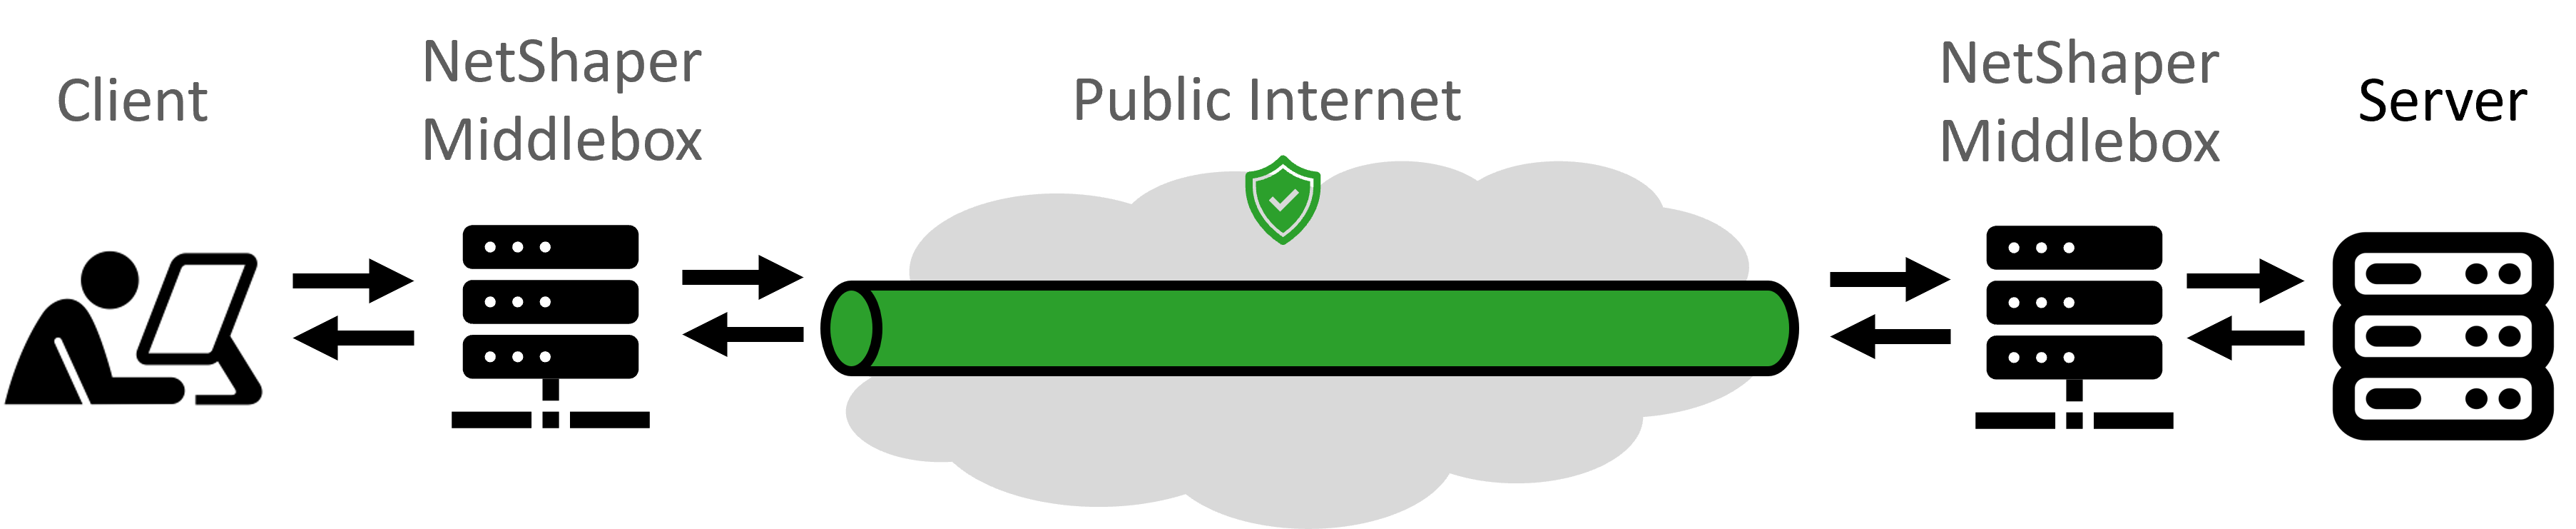
\includegraphics[width=\columnwidth]{figures/netshaper/netshaper-setup.png}
    \caption{NetShaper's Tunnel Setup}
    \label{fig:netshaper-setup}
\end{figure}

We designed NetShaper as a modular system that can be deployed using a pair of middleboxes, forming a forward and reverse proxy pair (see \Cref{fig:netshaper-setup}). 
Here, we describe in detail the architecture of the proxy setup and defer the discussion regarding the design of the middlebox to \Cref{sec:netshaper-middlebox-design}. 

When using NetShaper, all clients communicate with the servers using three piecewise connections: 
(\textit{i}) between the client and the client-side middlebox, 
(\textit{ii}) between the client-side middlebox and the server-side middlebox, and
(\textit{iii}) between the server-side middlebox and the server.

For connection \textit{i} and \textit{iii}, NetShaper relies on standard TCP/UDP protocols. However, for connection \textit{ii} (i.e. to proxy the payload), NetShaper utilises QUIC. 
Using QUIC to proxy the payload avoids the TCP meltdown problem [??] that occurs when tunnelling TCP via TCP.
In addition, using QUIC also avoids the problem of an observer/attacker being able to distinguish between payload and padding that would occur when TCP was tunnelled via UDP (as the end host would retransmit payload, but the padding would not be retransmitted).

\paragraph{Setup.}
In order to be able to proxy end host traffic via NetShaper, the middleboxes need to be configured. 
The middleboxes first establish an encrypted QUIC connection between them, with user-specified reliability semantics.
Once the QUIC connection is established, NetShaper initialises three types of QUIC streams: Control, Data (Payload), and Dummy (Padding).
One \textit{control} stream is used to transmit messages regarding connection establishment or termination by the end host.
One \textit{dummy} stream is used for adding padding to the payload whenever necessary, based on the output of $f_{DP}$
\footnote{We avoid the use of PADDING frames in QUIC as they do not elicit acknowledgements and hence are distinguishable from the payload \cite{quic_rfc}.}.

\paragraph{Supporting multiple end hosts.}
As we discussed in \Cref{subsec:netshaper-background-quic}, QUIC supports multiple streams in the same connection.
Using this, NetShaper can proxy the payload of multiple end hosts through a single QUIC connection between a pair of middleboxes.

While QUIC can support arbitrary initialisation and termination of streams, each stream has an associated header, which would increase the total transmission size.
For example, when transmitting two bytes in a single stream, the total transmission size would be $2 + S_{header}$.
However, when transmitting two streams of one byte each, the total transmission size would be $2 + 2*S_{header}$. 
An adversary may be able to distinguish between these two scenarios.
In order to avoid such a situation, NetShaper fixes and initialises a fixed number of streams per QUIC connection during the setup phase.
NetShaper assigns an unused stream to the client whenever a new client connects to the middlebox.
Similarly, NetShaper marks a stream as unused when an end host terminates the connection.

\endinput
\section{Middlebox Design}
\label{sec:netshaper-middlebox-design}

While it is possible to apply NetShaper framework's approach at any network layer, we chose to develop the system as an L4 (Transport Layer) proxy.
This enables the system to be easily deployable, entirely in userspace and without requiring any superuser privileges. 
Developing NetShaper at L2 (Data Link Layer) or L3 (Network Layer) would require the deployer to either have the ability to modify the OS kernel or deploy some form of kernel bypass.

\begin{figure}[!htb]
    \centering
    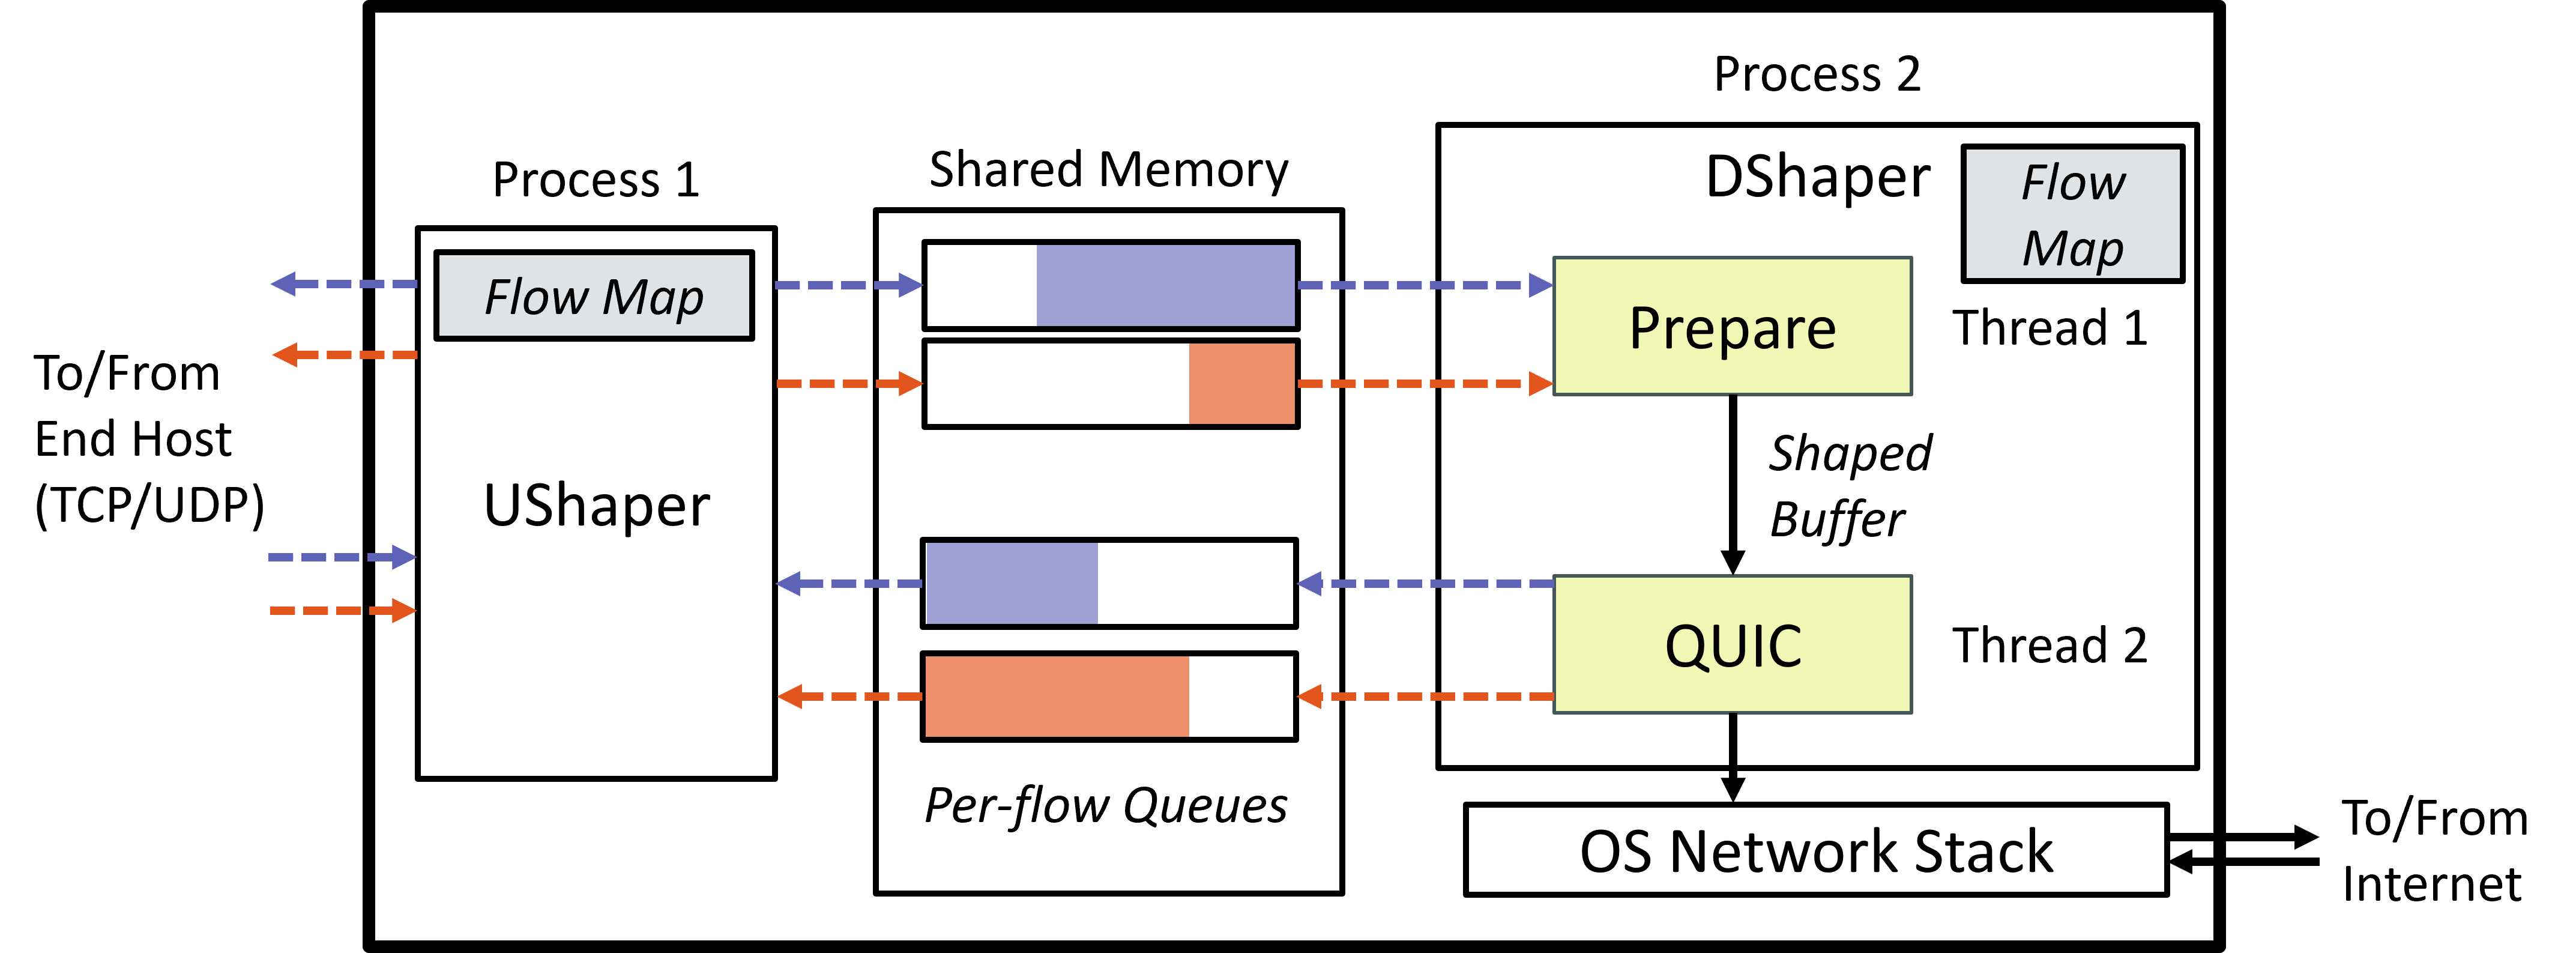
\includegraphics[width=\columnwidth]{figures/netshaper/middlebox-design.png}
    \caption{NetShaper Middlebox Design}
    \label{fig:middlebox-design}
\end{figure}

As outlined in \Cref{fig:middlebox-design}, NetShaper's middlebox consists of two main processes: UShaper and DShaper, and a shared memory between them.

\paragraph{UShaper.}
The \textit{UShaper} implements a client or a server to communicate with the end host.
It shares some Lamport Queues (LQs) [??] with DShaper.
It also consists of a flow map that maps a client with a corresponding pair of LQs.
\textit{UShaper} updates the flow map whenever a client establishes or terminates a connection.
In addition, it assigns an unused pair of LQs (one outbound and one inbound) to a new client and revokes that whenever the client terminates the connection.
The \textit{UShaper} receives outbound traffic from the end host and enqueues the payload in the assigned LQ.
Similarly, it dequeues inbound traffic from the inbound LQs and sends it to the corresponding end hosts.

\paragraph{DShaper.}
The \textit{DShaper} consists of two threads: \textit{Prepare} and \textit{QUIC worker}, and a flow map.
The flow map maps an LQ with a pre-initialised QUIC stream.
The \textit{Prepare} thread also measures the data available in the outbound LQs at the start of the window $W$.
It then adds noise to this available size based on the DP parameters.
Finally, it enqueues the payload and padding that needs to be transmitted.
The \textit{QUIC worker} transmits the enqueued data out to the network.
It also processes the received data, places it in the relevant LQ, and updates the flow map whenever a client initialises or terminates a connection.

In order to ensure that the operation of \textit{UShaper}, \textit{Prepare}, and \textit{QUIC worker} do not interfere with each other, we apply a few constraints in the implementation, and during the deployment of NetShaper.
First, all three components are required to be pinned on separate cores so that the execution time of one may not impact the others.
Second, in order to not leak the size of the payload due to the processing time of the enqueue operation done by the \textit{Prepare} thread, the \textit{Prepare} thread applies a lock for a fixed duration, during which the \textit{QUIC worker} can not transmit the data. 
We have outlined pseudo-code for both prepare and QUIC worker in \Cref{lst:prepare_and_worker}.
Finally, when receiving data, the \textit{QUIC worker} also enqueues the dummy bytes to a designated LQ so that the processing time remains consistent with the size of the data (see Figure ??).

\paragraph{Shared Memory.}
Both \textit{UShaper} and \textit{DShaper} have a shared memory between them.
This shared memory consists of three types of LQs: Control, Payload, Dummy
Similar to the stream types outlined in \Cref{sec:netshaper-proxy-arch}, \textit{Control} LQ transmits the information about a connection establishment or termination by a client. 
\textit{Payload} LQ consists of the bytes received from the end host or to be sent to the end host.
\textit{Dummy} LQ consists of the dummy/padding bytes that are received.

\begin{minipage}{\textwidth}
\lstinputlisting[language=Python]{code/netshaper/prepare_and_worker.py}
\captionsetup{type=lstlisting}
\caption{Prepare and QUIC Worker Pseudo-code}
\label{lst:prepare_and_worker}
\end{minipage}

\endinput


\begin{figure}[!htb]
    \centering
    
\includegraphics[width=\columnwidth]{figures/netshaper/middlebox-design-overview.png}
    \caption{Overview of NetShaper's Middlebox}
    \label{fig:middlebox-design-overview}
\end{figure}

\endinput

Should we add pseudo-codes for UShaper and DShaper?
\section{Evaluation}
\label{sec:netshaper-evaluation}

We evaluate NetShaper on a variety of performance metrics.
First, we evaluate the peak line rate that NetShaper can support. 
Next, we evaluate the maximum throughput that the NetShaper middlebox can sustain.
Then, we measure the latency that NetShaper's middlebox will incur without any traffic shaping.
And finally, we measure the relation between NetShaper's latency and $W$ when traffic is being shaped.

\subsection{Setup}
\label{subsec:netshaper-evaluation-setup}

\begin{figure}[!htb]
    \centering
    
\includegraphics[width=\columnwidth]{figures/netshaper/testbed-setup.png}
    \caption{Evaluation Setup}
    \label{fig:testbed-setup}
\end{figure}

Our setup consists of four desktops, each of which consists of 32GB RAM, 1TB storage, one Marvell AQC113CS-B1-C 10G NIC, and one Realtek RTL8111 1G NIC.
We use the Realtek NIC only as a management NIC and do not run any experiments on it.
Three of the desktops have an AMD Ryzen 7 7700X processor, and one has a more powerful AMD Ryzen 9 7900X processor, which we use as the server.
The middleboxes are connected to each out via an additional Intel X550-T2 10G NIC.
The client and the server are connected to their local middleboxes via the Marvell 10G NIC.
This forms a linear topology, as outlined in \Cref{fig:testbed-setup}
All the desktops run Ubuntu 22.04.02 (linux kernel version 5.19)

All of our experiments contain a baseline setup (\textbf{Base}) wherein the client is directly connected to the server via the Marvell 10G NIC, bypassing the middleboxes.

\begin{comment}

Mention iperf, wrk2 (modified), nginx?
Maybe here maybe in the experiments themselves

\end{comment}
\subsection{max \#packets}
\label{subsec:netshaper-evaluation-max-packets}
\subsection{max throughput}
\label{subsec:netshaper-evaluation-max-throughput}
% \subsection{minimum DShaper loop duration}
\label{subsec:netshaper-evaluation-minimum-dshaper-loop-duration}
\subsection{impact of dshaper loop duration}
\label{subsec:netshaper-evaluation-impact-of-dshaper-loop-duration}
\section{Limitations}
\label{sec:netshaper-limitations}

Our implementation has two security limitations.
First, it relies on the MSQUIC implementation of QUIC, which utilises OpenSSL, which may not provide constant time cryptography.
However, this limitation can be easily remedied by modifying MSQUIC so that it uses a constant-time cryptography library such as WolfSSL \cite{wolfssl}.
Second, it is difficult to profile for $T_{prep}$ and $T_{enq}$. 
If the time taken by the \textit{Prepare} thread exceeds that of the profiled values, it violates our theoretical DP guarantees. 
However, in practice, it is difficult to exploit these violations for carrying out traffic analysis based network side-channel attacks.

NetShaper has two more limitations in terms of usability and performance.
First, we currently require a custom configuration format supplied by the client to configure the destination for a connection. 
However, given the modular architecture of our system, one can easily implement \textit{UShaper} as a SOCKS5 proxy \cite{leech1996socks} or any other standard proxy protocol.
Second, the current implementation dedicates only one core each to \textit{UShaper}, \textit{Prepare}, and \textit{QUIC Worker}. These can become a bottleneck. 
While it is relatively simple to dedicate more cores for \textit{UShaper} or \textit{QUIC Worker}, doing so for the \textit{Prepare} thread is non-trivial, as it has to aggregate data from all the available clients.
\section{Related Work}
\label{sec:netshaper-related-work}

While prior work has explored various approaches for mitigating network side-channel attacks, most focus on conceptual methods, with only a few providing a practical system to address the issue.
CS-BuFLO \cite{cai2014csbuflo} applies traffic shaping by transmitting a fixed number of bytes at semi-regular intervals while remaining receptive to congestion control.
DeltaShaper \cite{barradas2017deltashaper} obfuscates the traffic shape to always look like a video conference stream.
It transcodes the application traffic as a video stream that is then fed to Skype with a virtual camera.
While both implementations require modifications to the end hosts, their approach can conceptually be implemented as a middlebox.
However, their approach is not adaptive to the application traffic and, hence, can result in either high bandwidth overhead or high latency.
In addition, DeltaShaper is also unable to support more than one application stream at a time.
HTTPOS \cite{luo2011httpos}, ALPaCA and LLaMA \cite{cherubin2017llama}, and Walkie-Talkie \cite{wang2017walkie} all require modification of the end-hosts and support only HTTP applications.

Pacer \cite{mehta2022pacer} provides a shaping tunnel that is conceptually similar to NetShaper's tunnel design (see \Cref{sec:netshaper-designing-traffic-shaping-tunnel}).
However, Pacer protects a cloud tenant's data from being leaked to a co-located adversary via congestion in a shared network link.
As such, Pacer controls the transmit time of TCP packets based on the shaping schedule and congestion control signals.
Achieving this requires non-trivial modifications to the end-hosts.
On the other hand, NetShaper protects applications in different private networks that are communicating over the public internet. 
As such, NetShaper can be placed as a gateway for the private networks to access the public internet, thus requiring none to minimal changes on the end-hosts.
In addition, NetShaper's approach requires precise timing only for the generation of bursts of DP length and not for the actual network transmission, requiring no modification of the underlying network stack.

QCSD \cite{smith2022qcsd} shares similarities with NetShaper, as both rely on the QUIC protocol. 
However, QCSD requires modifications to the client-side browser, unlike NetShaper. 
Since no server-side modifications are necessary, QCSD depends on the client to control the amount of data sent by the server, including the addition of padding or dummy bytes.
This approach requires the client to be aware of the sizes of the content the server hosts, as otherwise, the client may request more padding/dummy bytes than the requested content contains.
In addition, their approach does not scale well with an increasing number of client applications, as each client application will require its own QUIC connection, which in turn results in per-client dummy/padding bytes being transferred.

Ditto \cite{meier2022ditto} and NetShaper both shape traffic at network nodes that do not coincide with the end-hosts.
However, NetShaper's approach is hardware-independent, modular, and portable.
As such, NetShaper can be integrated into routers, gateways, end-hosts, and even programmable switches such as the one on which Ditto was deployed.



\endinput